% !TeX root = ../MSc.tex
\newcommand{\vv}{v_0}
\newcommand{\OriginalName}{(1,1.5),(2,1),(3,2.5),(4,1.5)}
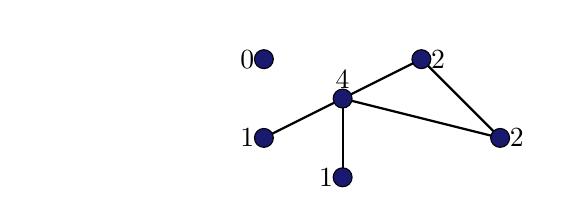
\begin{tikzpicture}[scale=1] 
\clip (-2,2.9) rectangle(4.5,0.8);
\coordinate (V) at (2,2);
\foreach \coord in \OriginalName{\draw[thick] (V) --\coord;}
\draw[thick](4,1.5)-- (3,2.5);
\draw[fill=MidnightBlue] (1,2.5) circle(0.12)node[left]{0};
\draw[fill=MidnightBlue] (V) circle(0.12)node[above]{4};
\draw[fill=MidnightBlue] (1,1.5) circle(0.12) node[left]{1};
\draw[fill=MidnightBlue] (2,1) circle(0.12) node[left]{1};
\draw[fill=MidnightBlue] (3,2.5) circle(0.12) node[right]{2};
\draw[fill=MidnightBlue] (4,1.5) circle(0.12) node[right]{2};
\end{tikzpicture}%
\begin{tikzpicture}[scale=1] 
\clip (-2,2.9) rectangle(6.5,0.8);
\coordinate (V) at (2,2);
\foreach \coord in \OriginalName{\draw[thick, -{Latex[length=4mm, width=2mm]}] (V) --\coord;}
\draw[thick, -{Latex[length=4mm, width=2mm]}](4,1.5)-- (3,2.5);
\draw[fill=MidnightBlue] (1,2.5) circle(0.12)node[left]{0/0};
\draw[fill=MidnightBlue] (V) circle(0.12)node[above]{0/4};
\draw[fill=MidnightBlue] (1,1.5) circle(0.12) node[left]{1/0};
\draw[fill=MidnightBlue] (2,1) circle(0.12) node[left]{1/0};
\draw[fill=MidnightBlue] (3,2.5) circle(0.12) node[right]{2/0};
\draw[fill=MidnightBlue] (4,1.5) circle(0.12) node[right]{1/1};
\end{tikzpicture}
%\caption{Undirected graph with degree centrality on the left, directed graph with in-degree/out-degree centrality on the right. Note that the sum $C_{D} = C_{Di} + C_{Do}$ for each vertex is the value of  the corresponding vertex on the graph on the left.}